\documentclass[5p]{elsarticle}
\bibliographystyle{elsarticle-num}

% encoding and language
\usepackage[utf8]{inputenc}
\usepackage[T1]{fontenc}
\usepackage[english]{babel}
\usepackage[babel]{csquotes}

% graphics support
\usepackage{graphicx}
\usepackage{epsfig}
\usepackage{float}
\usepackage{color}

% nice tables
\usepackage{booktabs}

% hyperrefs
\usepackage{hyperref}


\begin{document}

\begin{frontmatter}
	\title{Report: Correlations of Sample Quality and Functional Enrichment in ChIP-Seq Experiments}
	\author{Jannik Möllmann, Student M.Sc. Applied Bioinformatics}

	\begin{abstract}
		This report sums up the work and results of a practical research internship, I took under the guidance of Dr. Jean-Fred Fontaine from April 2020 to September 2020 in the group of Prof. Andrade at the Johannes-Gutenberg-University in Mainz, Germany. Although numerous approaches to characterize the potential biases involved in NGS data have been undertaken, there does not seem to be a clear understanding of the biases introduced by the expression of specific genes and pathways \cite{chen_systematic_2012,cheung_systematic_2011,park_widespread_2013,ramachandran_bidchips_2015,teng_accounting_2017,wang_correcting_2017}. Therefore the focus of the following investigations is to try to elucidate these biases for ChIP-seq data. The investigations relied on quality scores assigned to each sample with a novel quality control tool \cite{albrecht_automated_2020} and then split into three different paths, correlating the scores to 1) the disease state of the ChIP-seq samples 2) individual batches of ChIP-seq peaks of length 1000bp along the genome and 3) to pathways retrieved through functional enrichment analysis. Although, the size of the analysis of 11 datasets is still too small to get results of sufficient statistical significance and we had to focus on only one histone mark (H3K27ac), the results already show an unequal distribution of positively and negatively correlated genes and pathways, suggesting that there may be non-random variation in expression profiles between different samples of different experimental conditions. 
	\end{abstract}
\end{frontmatter}


\section{Materials and Methods}

\subsection{Data Retrieval and Annotation}
The data of this analysis was retrieved from the Gene Expression Omnibus database between April and July of 2020. In an earlier part of the analysis, 7 human ChIP-seq datasets from experiments with diseased and healthy samples were selected, albeit targeting different histone marks. In the final part of the analysis, delivering the results shown here, 11 similar datasets were selected with the important difference of targeting the same histone mark (H3K27ac). All datasets were annotated using the Python library \textit{Pandas}, with a particular focus on extracting binary values of the healthy/disease state of each sample.

\begin{figure}[t] % place the figures at the top ([t]) or bottom ([b]) of the page or use a separate page ([p])
	\centering
	
	% replace the \rule line below by the following one to include an image from your file system and set the size constraint accordingly
	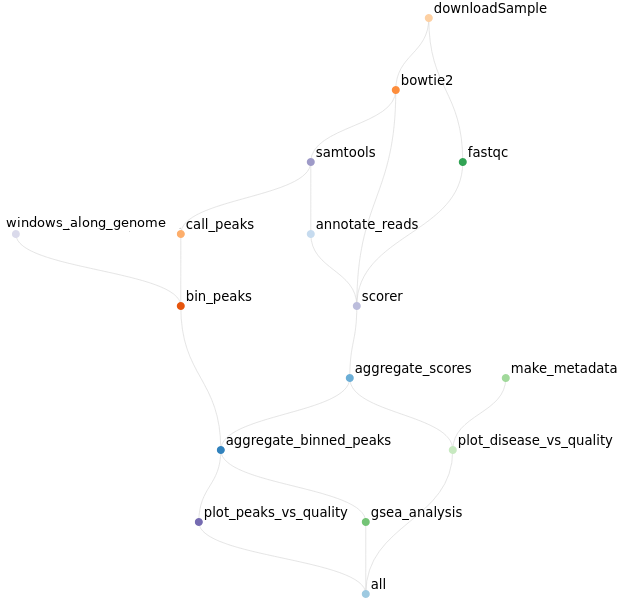
\includegraphics[width=250px]{../figures/workflow.png}
	
	\caption{Workflow of the Analysis. Each node in the graph represents one rule with each rule encapsulating a specific part of the analysis. The edges represent the dependencies between the rules with child rules (bottom nodes) depending on parent rules (top nodes). The analysis was thus ran from top to bottom with some rules performed more often than others (e.g. "gsea\_analysis" was performed only once while "downloadSample" was performed for each sample in the analysis).}
	\label{figure1}
\end{figure}

\subsection{Workflow}
The analysis performed here is based on an earlier analysis by Dr. Fontaine looking into RNA-seq data instead of ChIP-seq data. All individual steps of the analysis were assembled using \textit{SnakeMake} \cite{koster_snakemakescalable_2012}, allowing the analysis to be run in a closed environment in one piece and thus allowing for better reproducibility. The rules downloadSample, bowtie2, fastqc, annotate\_reads and scorer are mostly identical to the ones from the earlier analysis while the other rules were introduced specifically for this analysis. A graphical depiction of the workflow is shown in Figure \ref{figure1}.

\subsection{Quality Analysis}
The quality was analysed using the tool \textit{seqQScorer} \cite{albrecht_automated_2020} which incorporates the output from \textit{FastQC} as well as the un-annotated mapped reads and annotated mapped reads. The annotation of the reads was performed using an R script specifically provided for this purpose.

\subsection{Correlation of Disease State and Quality}
For each dataset a vector of binary values - indicating the disease state of each sample - and another vector of probability values - indicating the likelihood that the sample is of low quality - were brought together to calculate Pearson's product moment correlation coefficient and the accompanying p-value. The R code for this step can be found in the script "disease\_vs\_quality.r"

\subsection{Peak Calling}
Peaks were called using \textit{MACS2} on the mapped .bam files put out by the bowtie2 and samtools rules. No particular control files were given because of the heterogeneity of the control file information in the different datasets considered in this analysis. The standard padj-cutoff value of 0.05 as well as the narrow peak mode were used. The called peaks were put out in .bed format.

\subsection{Peak Binning}
For the binning of peaks along the whole genome the \textit{bedtools} tool suite \cite{quinlan_bedtools_2010} was used. First, the function \textit{makewindows} was used to make bins of 1000bp length and then the functions \textit{intersect}, \textit{groupby} and \textit{coverage} were used to count the number of peaks per bin and generate min, max and mean enrichment values for each bin.

\subsection{Correlation of Peak Bins and Quality}
For the correlation of peak bins and quality, only bins with peaks in at least 3 samples were considered and subsequently Pearson's product moment correlation coefficient was calculated four times - once for each metric (min, max, mean enrichment and peak count) - together with the vector of sample quality scores (already used for the correlation of disease state and quality). This step was performed in Python using the \textit{scipy} library and the code can be found in the files "aggregate\_binned\_peaks.py" and "quality\_vs\_peaks.py".

\subsection{Gene Set Enrichment Analysis}
For the gene set enrichment analysis, the KEGG subset of canonical pathways included in the MSig database version 7.1 was used along with the human reference genome hg38. For positive correlation coefficients a lower bound of 0.2 was set and for negative correlation coefficients an upper bound of -0.2, above and below which, respectively, bins were not considered for the gene set enrichment. The number of datasets that a particular bin was negatively or positively correlated in was counted by looping over all datasets with the \textit{countOverlaps} function from the \textit{GenomicRanges} R library. All bins passing the threshold were then annotated to the nearest transcription start site using the \textit{annotatePeaks} function from the \textit{ChIPseeker} R library \cite{yu_chipseeker_2015}. Since multiple bins were often annotated to the same gene, for each gene only the bin with the highest number of correlated datasets were considered. This then generated two tables assigning integer values between 0 and the number of datasets to each gene in the genome with one table for positively correlated genes and another table for negatively correlated genes. These two datasets could then be fed to the \textit{fgsea} function from the R library of the same name for automated gene set enrichment analysis \cite{korotkevich_fast_2019} together with the KEGG pathways described earlier and the parameters minSize = 15, maxSize = 500 and scoreType = "pos". 

\section{Results}

\subsection{Correlation of Disease State and Quality}
Out of 11 datasets, 4 datasets had a significant correlation between disease state and quality (p < 0.05). Out of these, one dataset with a very strong correlation coefficient and very low p-value (R = 0.747, p = 2.548e-13) turned out to be correlated due to a batch effect since the samples from the two groups were sequenced in two different labs with antibodies from two different providers. For the other three datasets such a straightforward explanation could not be found, suggesting that the correlations are due to actual differences in the quality of the samples of the two groups. All plots, each showing the correlation of the samples in a single dataset, are found as .png files in the folder "disease\_vs\_quality".

\begin{figure}[t] % place the figures at the top ([t]) or bottom ([b]) of the page or use a separate page ([p])
	\centering
	
	% replace the \rule line below by the following one to include an image from your file system and set the size constraint accordingly
	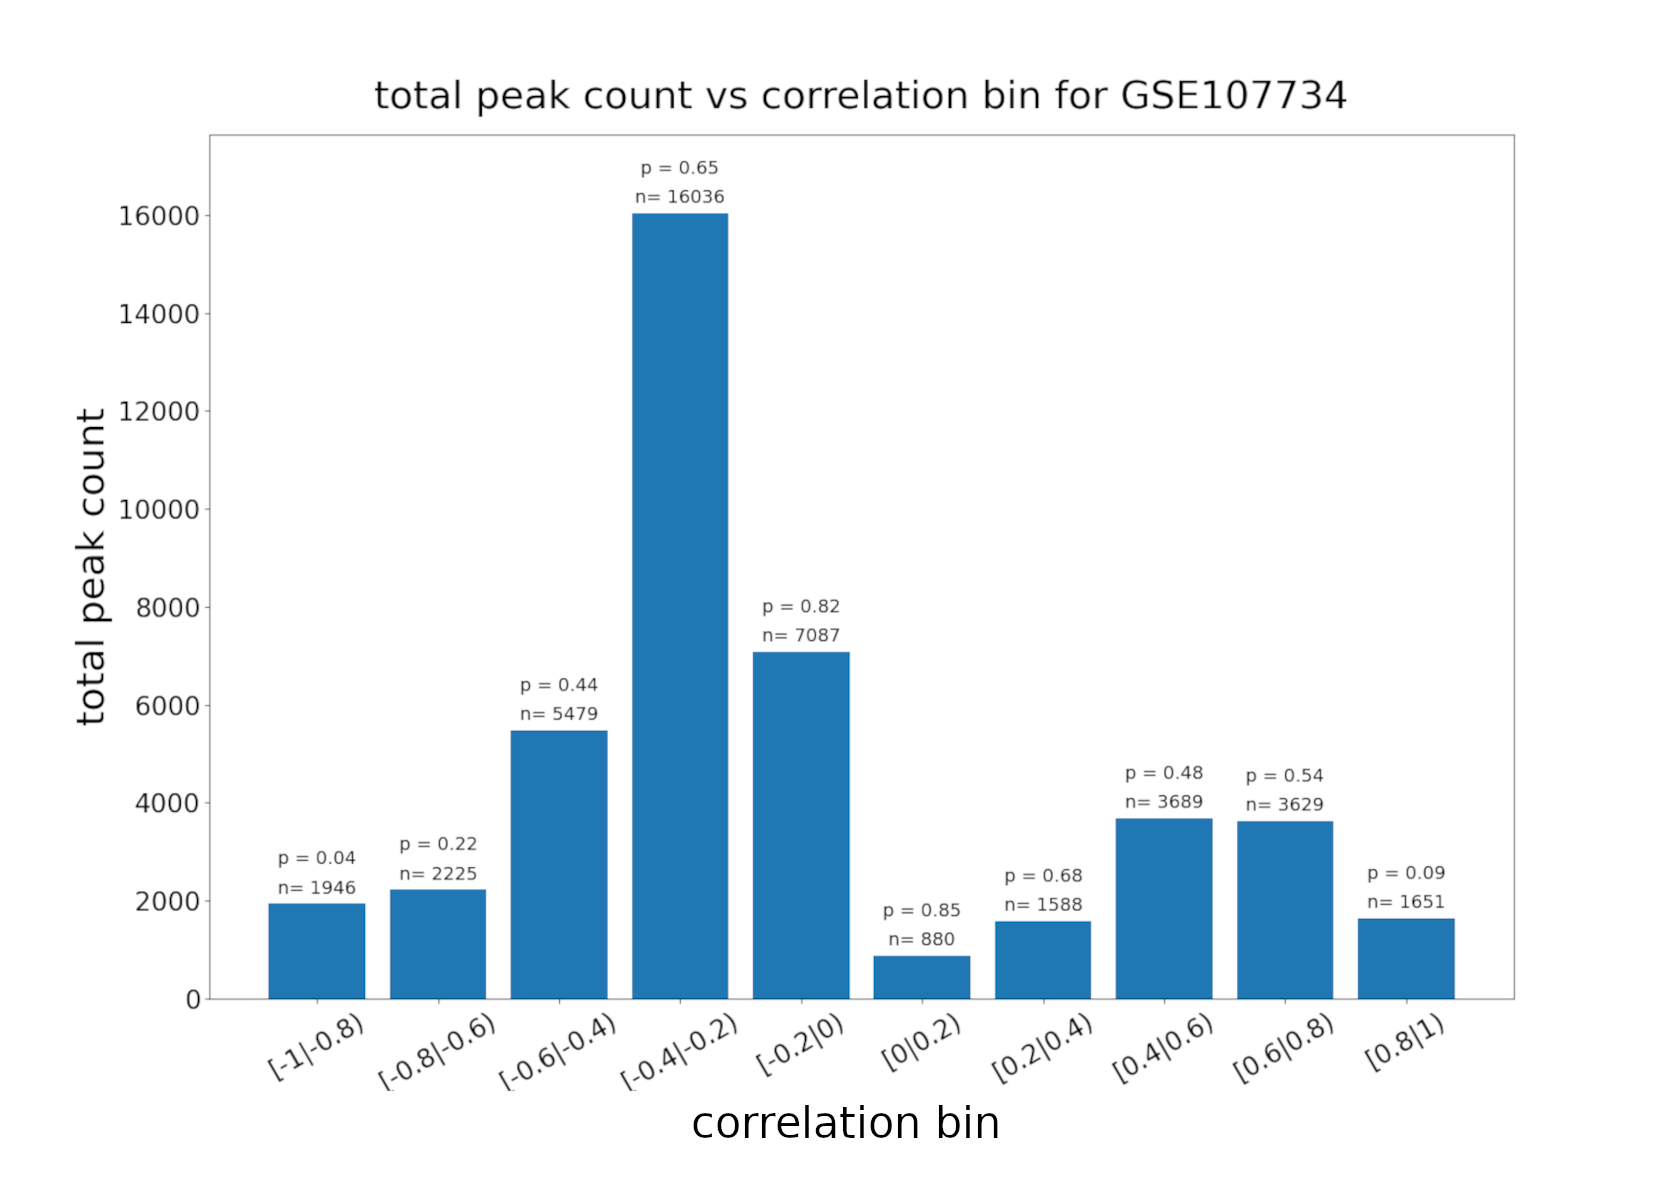
\includegraphics[width=250px]{../figures/peak_quality_corr_example.png}
	
	\caption{Exemplary Plot for the Correlation of Peak Count in Bins and Quality. The p-values above the bars are mean p-values over all correlation p-values in the given bin. N indicates the number of peaks falling into the given bin. The dataset in this example shows a bimodal distibution suggesting that this dataset splits into two groups of negatively and positively correlated peaks with the negatively correlated peaks more abundant than the positively correlated peaks.}
	\label{figure2}
\end{figure}

\subsection{Correlation of Peak Bins and Quality}
When plotting the correlation coefficients in 10 bins between -1 and 1 on the x-axis and the number of peaks in that correlation bin on the y-axis (or the min, max or mean enrichment of the peaks in the bin) the resulting distribution should give an intuition on wether there is a bias towards positively or negatively correlated peaks in a given dataset or if there is no bias (i.e. normally-distributed correlation coefficients). Figure \ref{figure2} shows an exemplary dataset with a slight bimodal distribution to explain the details of the plots. For most of the datasets however, there does not seem to be a clear deviation from the gaussian normal distribution curve suggesting that most datasets can not be split into two clear groups of positively and negatively correlated peaks or that they show any general bias towards positively or negatively correlated peaks. The dataset showing the most striking deviation from the normal distribution is the one portrayed in the figure (GSE107734). 

\begin{figure}[t] % place the figures at the top ([t]) or bottom ([b]) of the page or use a separate page ([p])
	\centering
	
	% replace the \rule line below by the following one to include an image from your file system and set the size constraint accordingly
	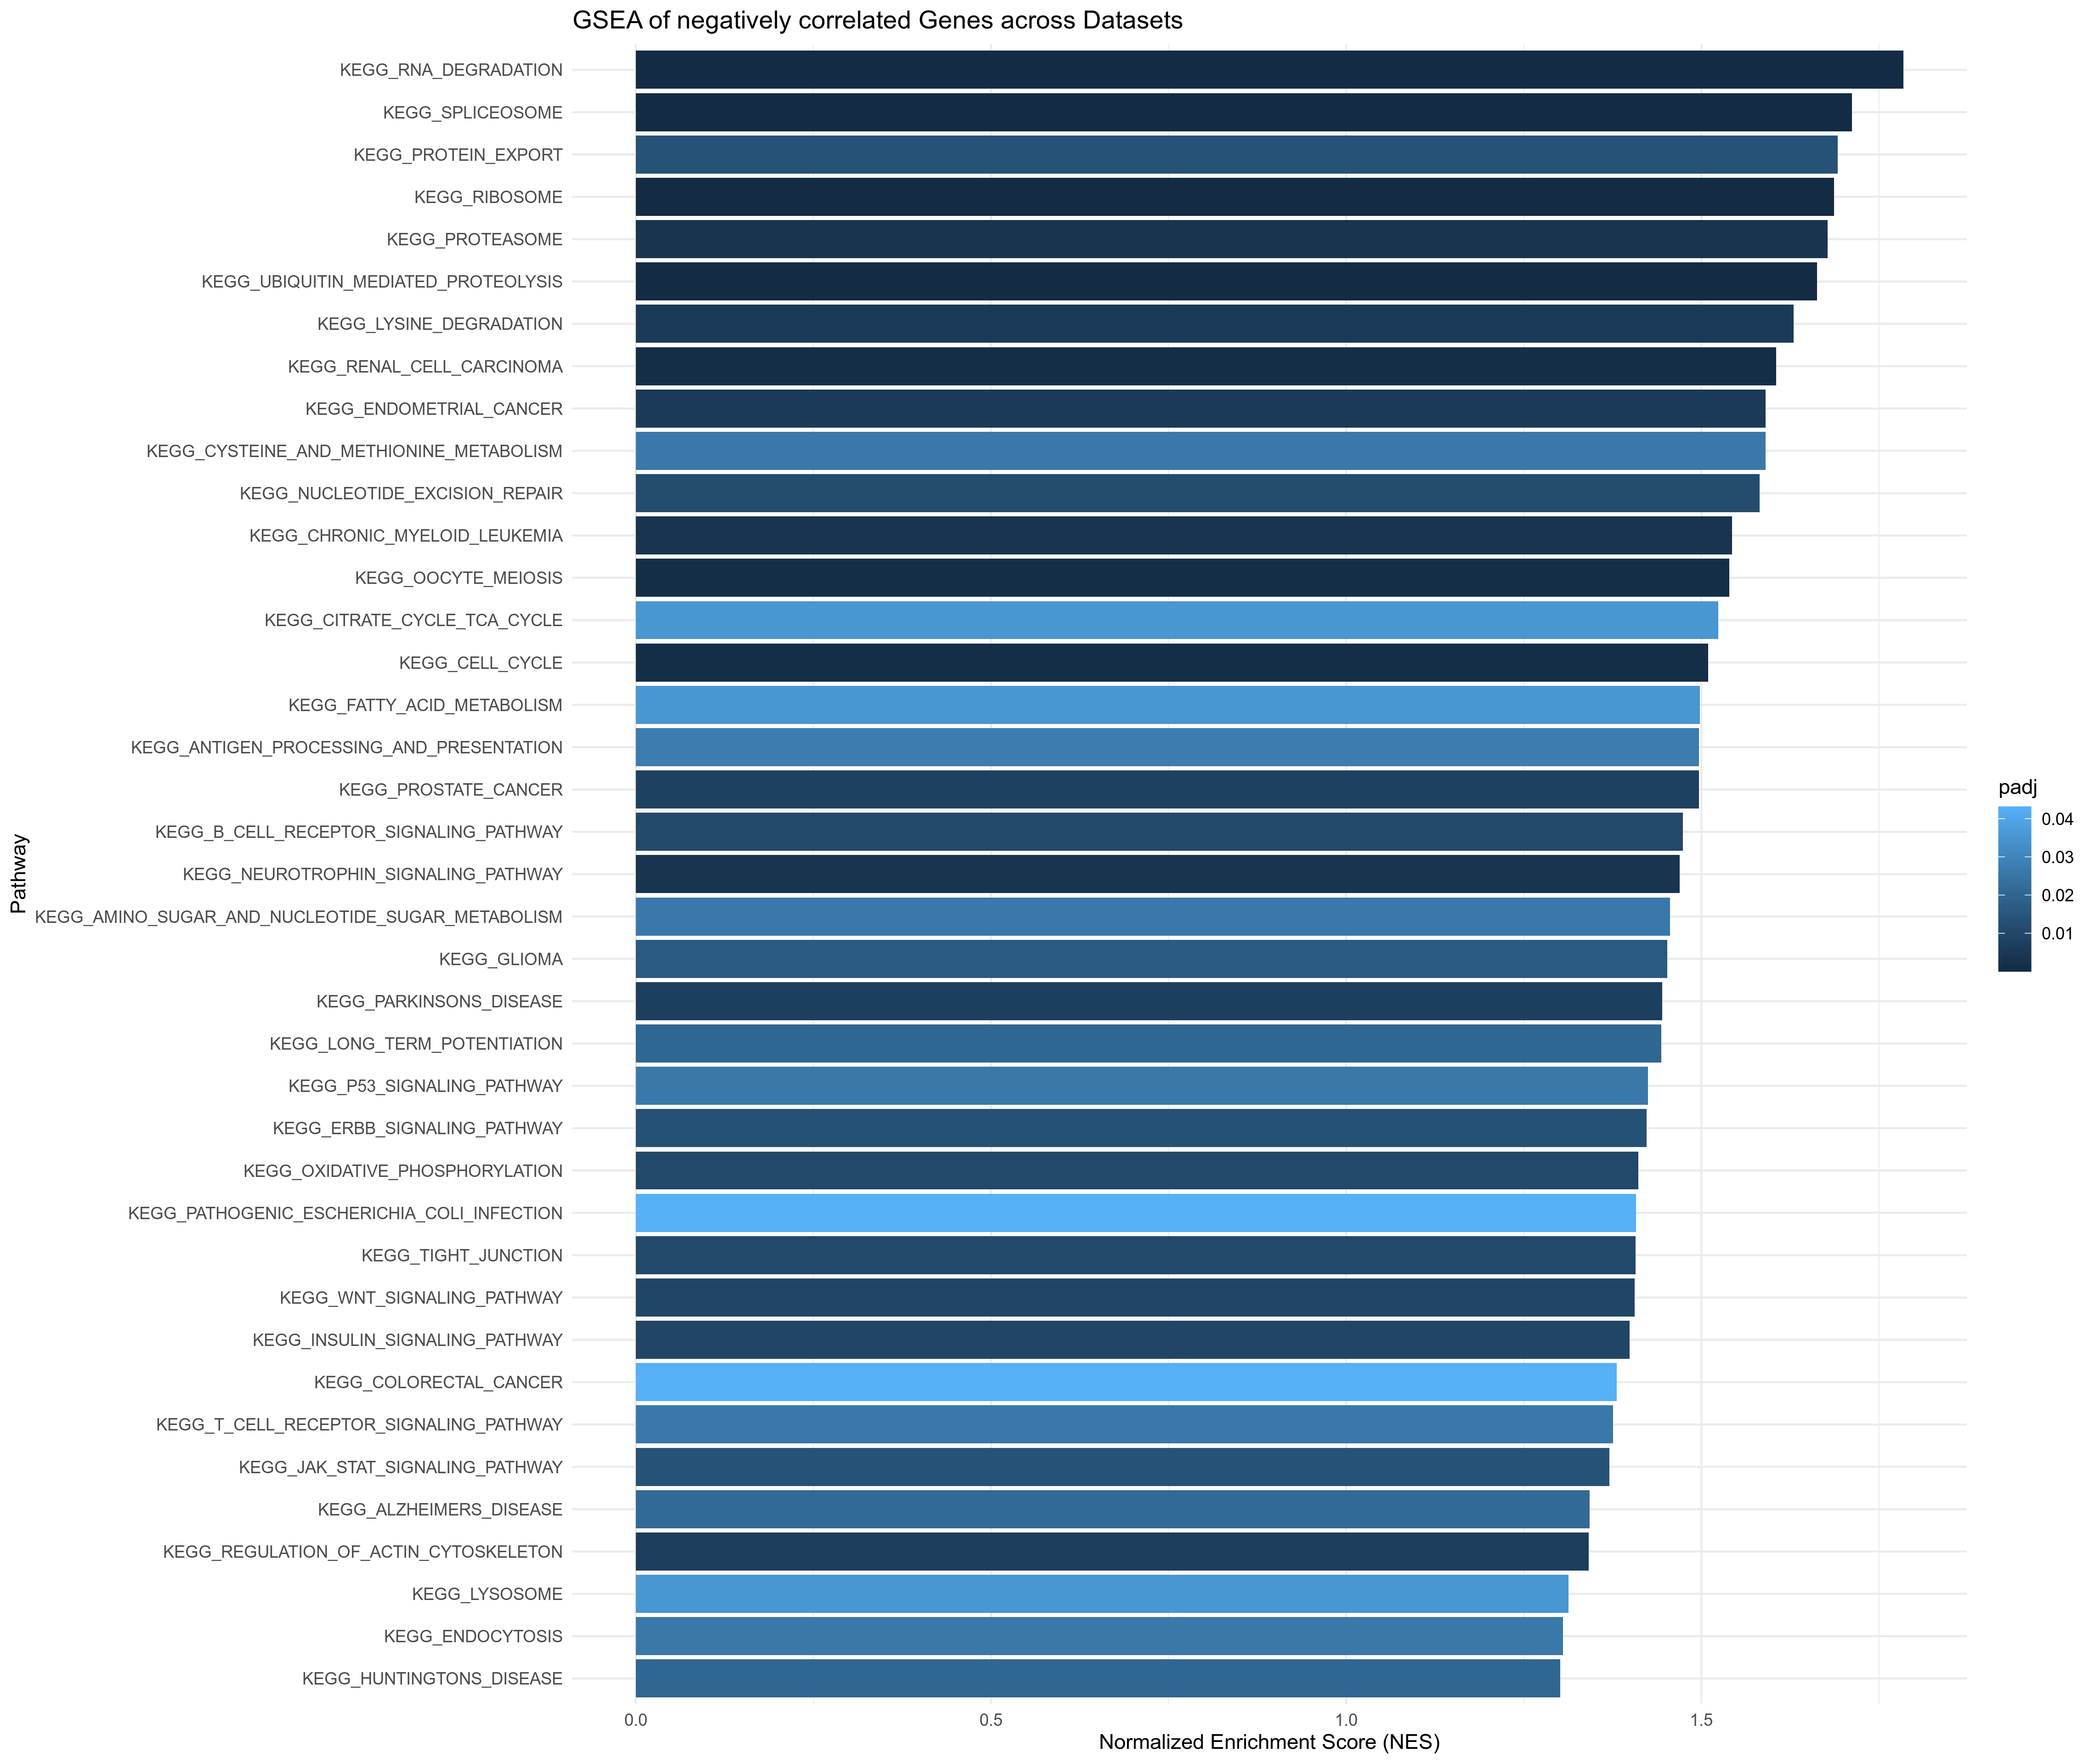
\includegraphics[width=250px]{../figures/negatively_correlated_pathways.png}
	
	\caption{Pathways Enriched in Negatively Correlated Genes. The figure shows the top 40 pathways significantly enriched in negatively correlated genes measured in terms of normalized enrichment score (NES). The colour indicates the significance value with darker colours representing more significant pathways.}
	\label{figure3}
\end{figure}

\begin{figure}[t] % place the figures at the top ([t]) or bottom ([b]) of the page or use a separate page ([p])
	\centering
	
	% replace the \rule line below by the following one to include an image from your file system and set the size constraint accordingly
	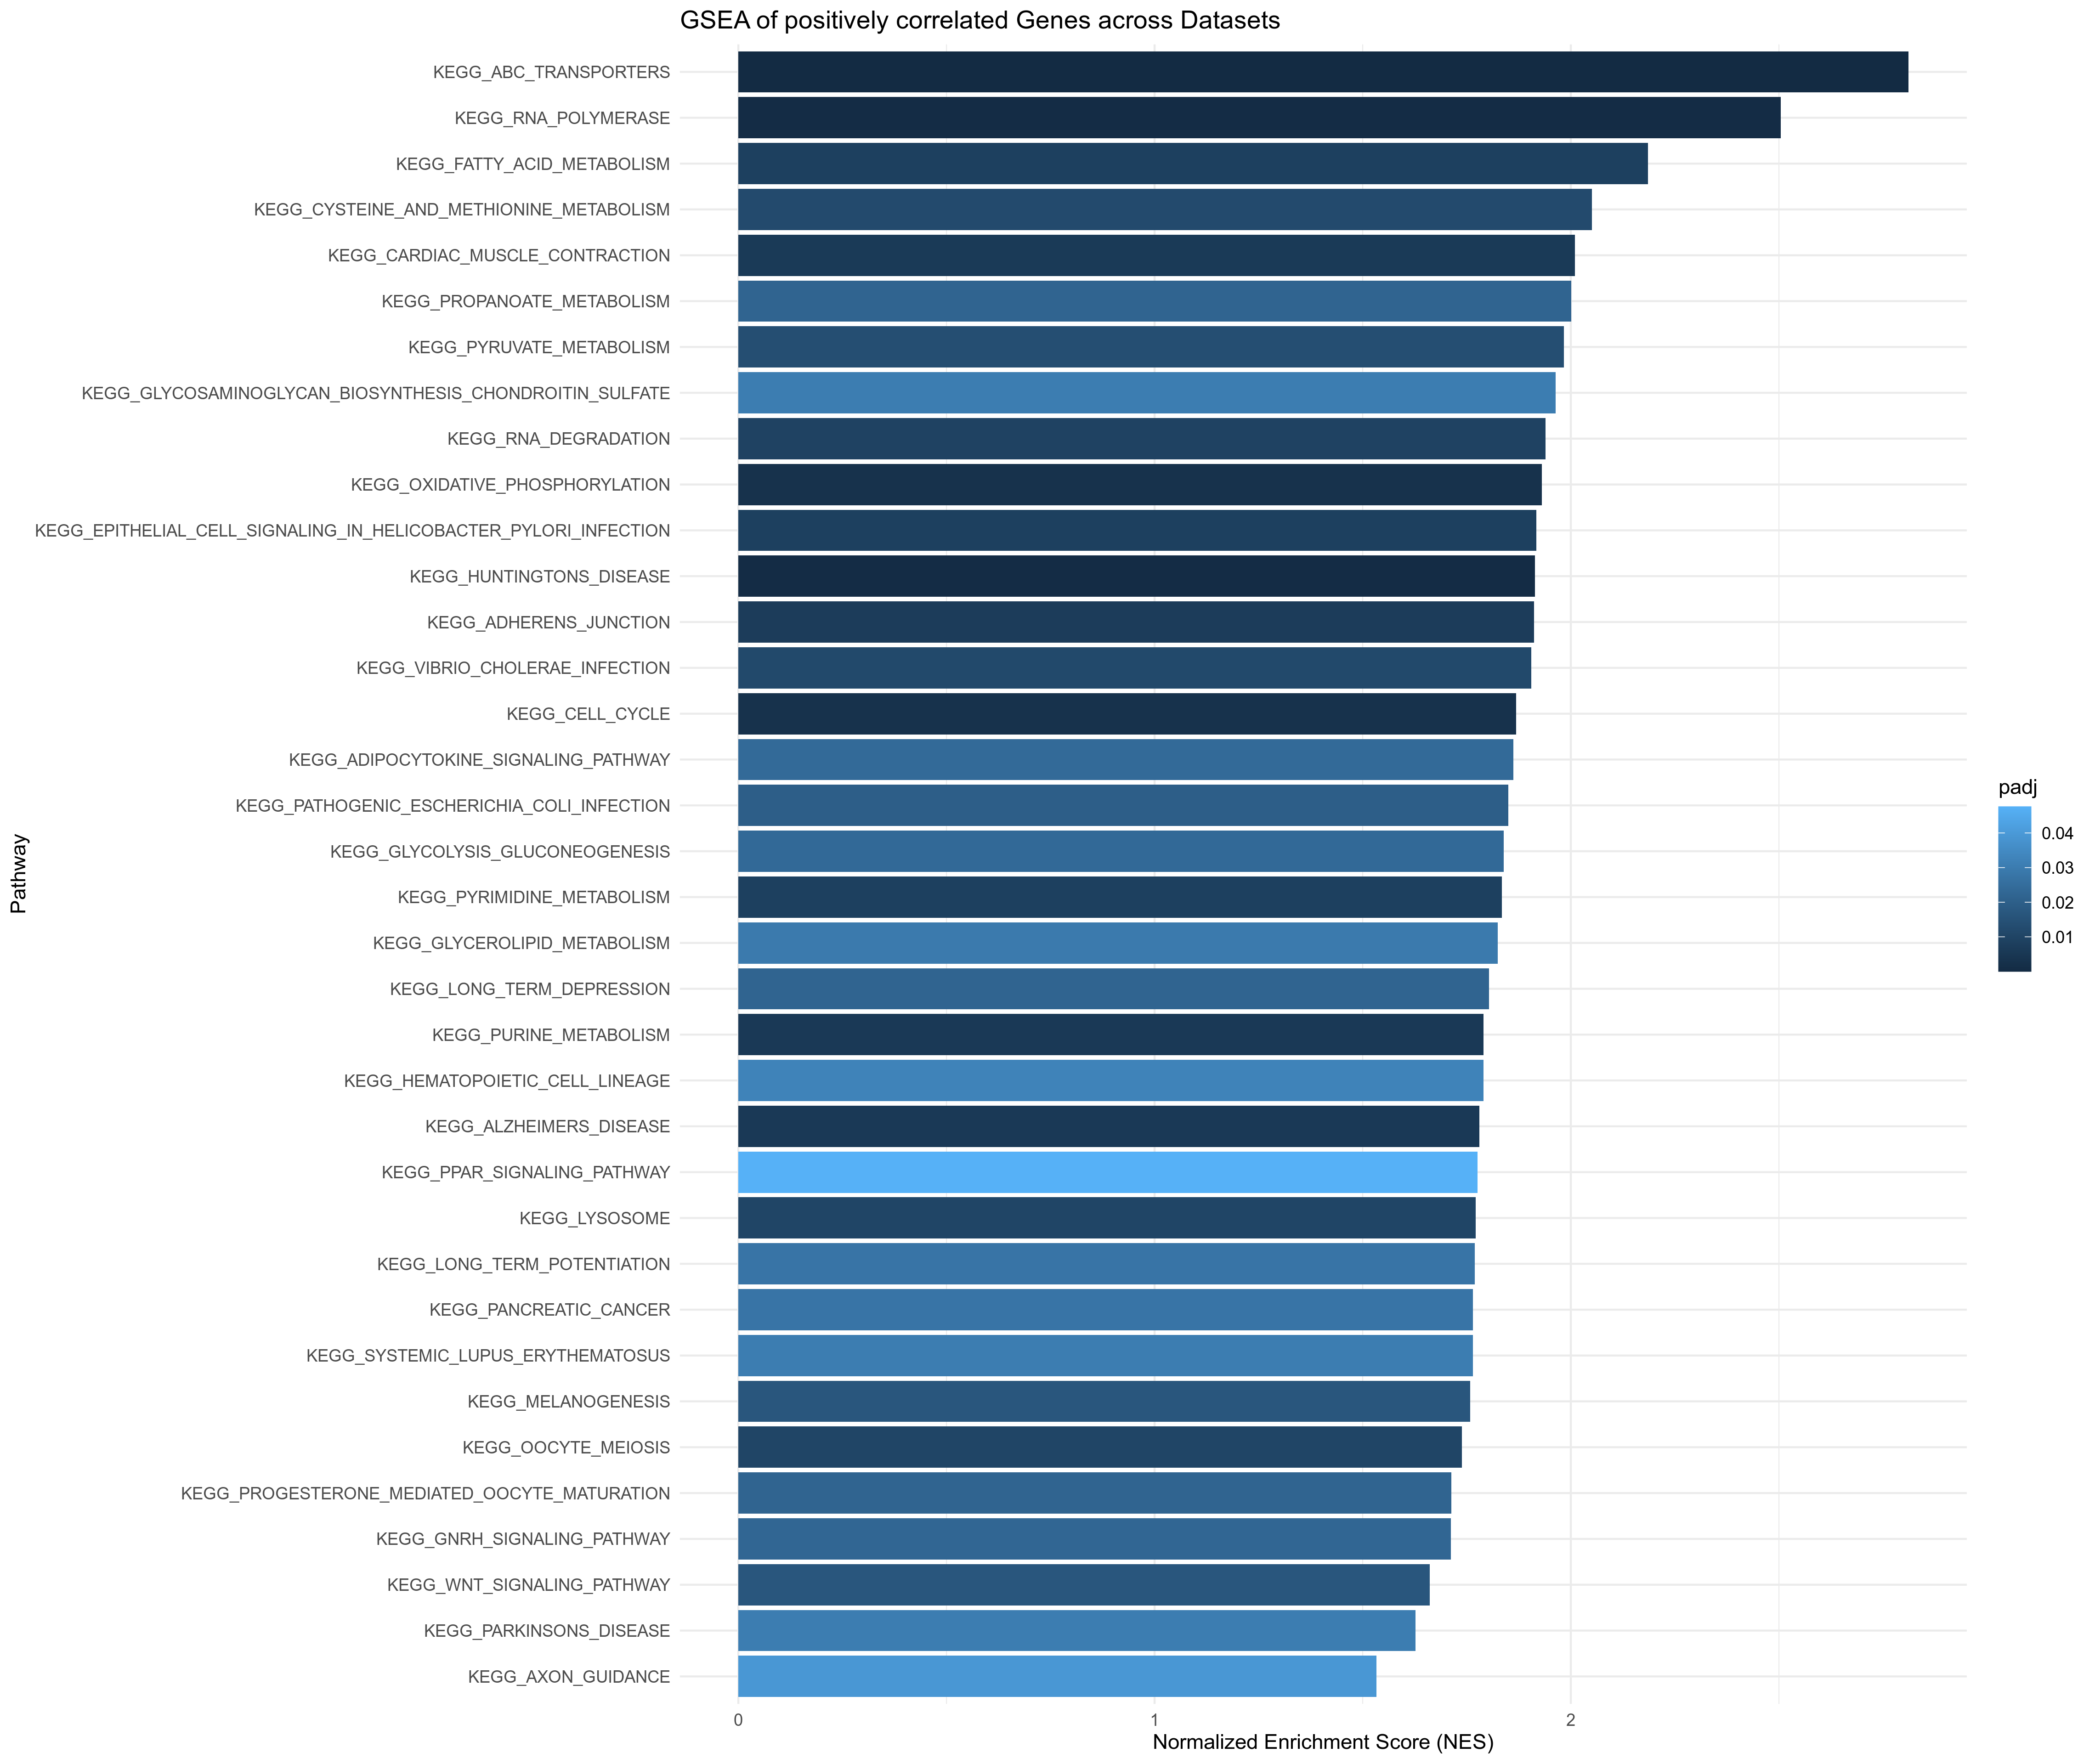
\includegraphics[width=250px]{../figures/positively_correlated_pathways.png}
	
	\caption{Pathways Enriched in Positively Correlated Genes. The figure shows the top 40 pathways significantly enriched in positively correlated genes measured in terms of normalized enrichment score (NES). The colour indicates the significance value with darker colours representing more significant pathways.}
	\label{figure4}
\end{figure}

\subsection{Gene Set Enrichment Analysis of Correlated Peaks}
When looking at the top negatively enriched pathways in Figure \ref{figure3} it seems striking that all of the top 7 pathways except for protein export are closely related to protein quality since they can all be grouped under either of the two categories protein production or protein degradation. A low protein quality can be expected to be detected by the novel quality control tool used here (seqQScorer) since it takes into account not just the raw reads but also the success in read mapping and the binding of reads to transcriptional start sites and other relevant genomic regions. This result thus seems to suggest that the tool has correctly identified samples that are of low quality due to cellular processes potentially lowering protein quality.

The top positively enriched pathways - shown in Figure \ref{figure4} - are more heterogenous with a high prevelance of primary metabolite synthesis pathways. However, it should be noted that the top two pathways are both related to protein quality.

\section{Conclusions}
 The results presented herein seem to suggest that 1) there exist unexplained associations between quality and disease state in some of the samples and that 2) there exist biases towards positively and negatively correlated genes in at least one of the samples and 3) the novel quality control tool used here worked as expected, detecting samples of low quality due to cellular processes affecting protein quality.

 However, the results presented herein are preliminary since the analysis was run under restricted conditions, i.e. with a randomly sampled subset of reads for every sample and a total number of datasets that is still too low for the gene set enrichment analysis.

\section*{References}
\bibliography{report} % compiled from "report.bib" using BibTeX

\end{document}